\chapter{Tabelle e Immagini}
\label{ch:third_chapter}
In questo capitolo ci saranno esempi di tabelle di grandi dimensioni e immagini disposte a griglia.

\section{Griglia 1x3}
Ecco un esempio di una griglia di immagini, come mostrato in Figura \ref{fig:fruit_images1x3}.
\begin{figure}[h!]
\centering

\begin{subfigure}[t]{0.30\textwidth}
  \centering
  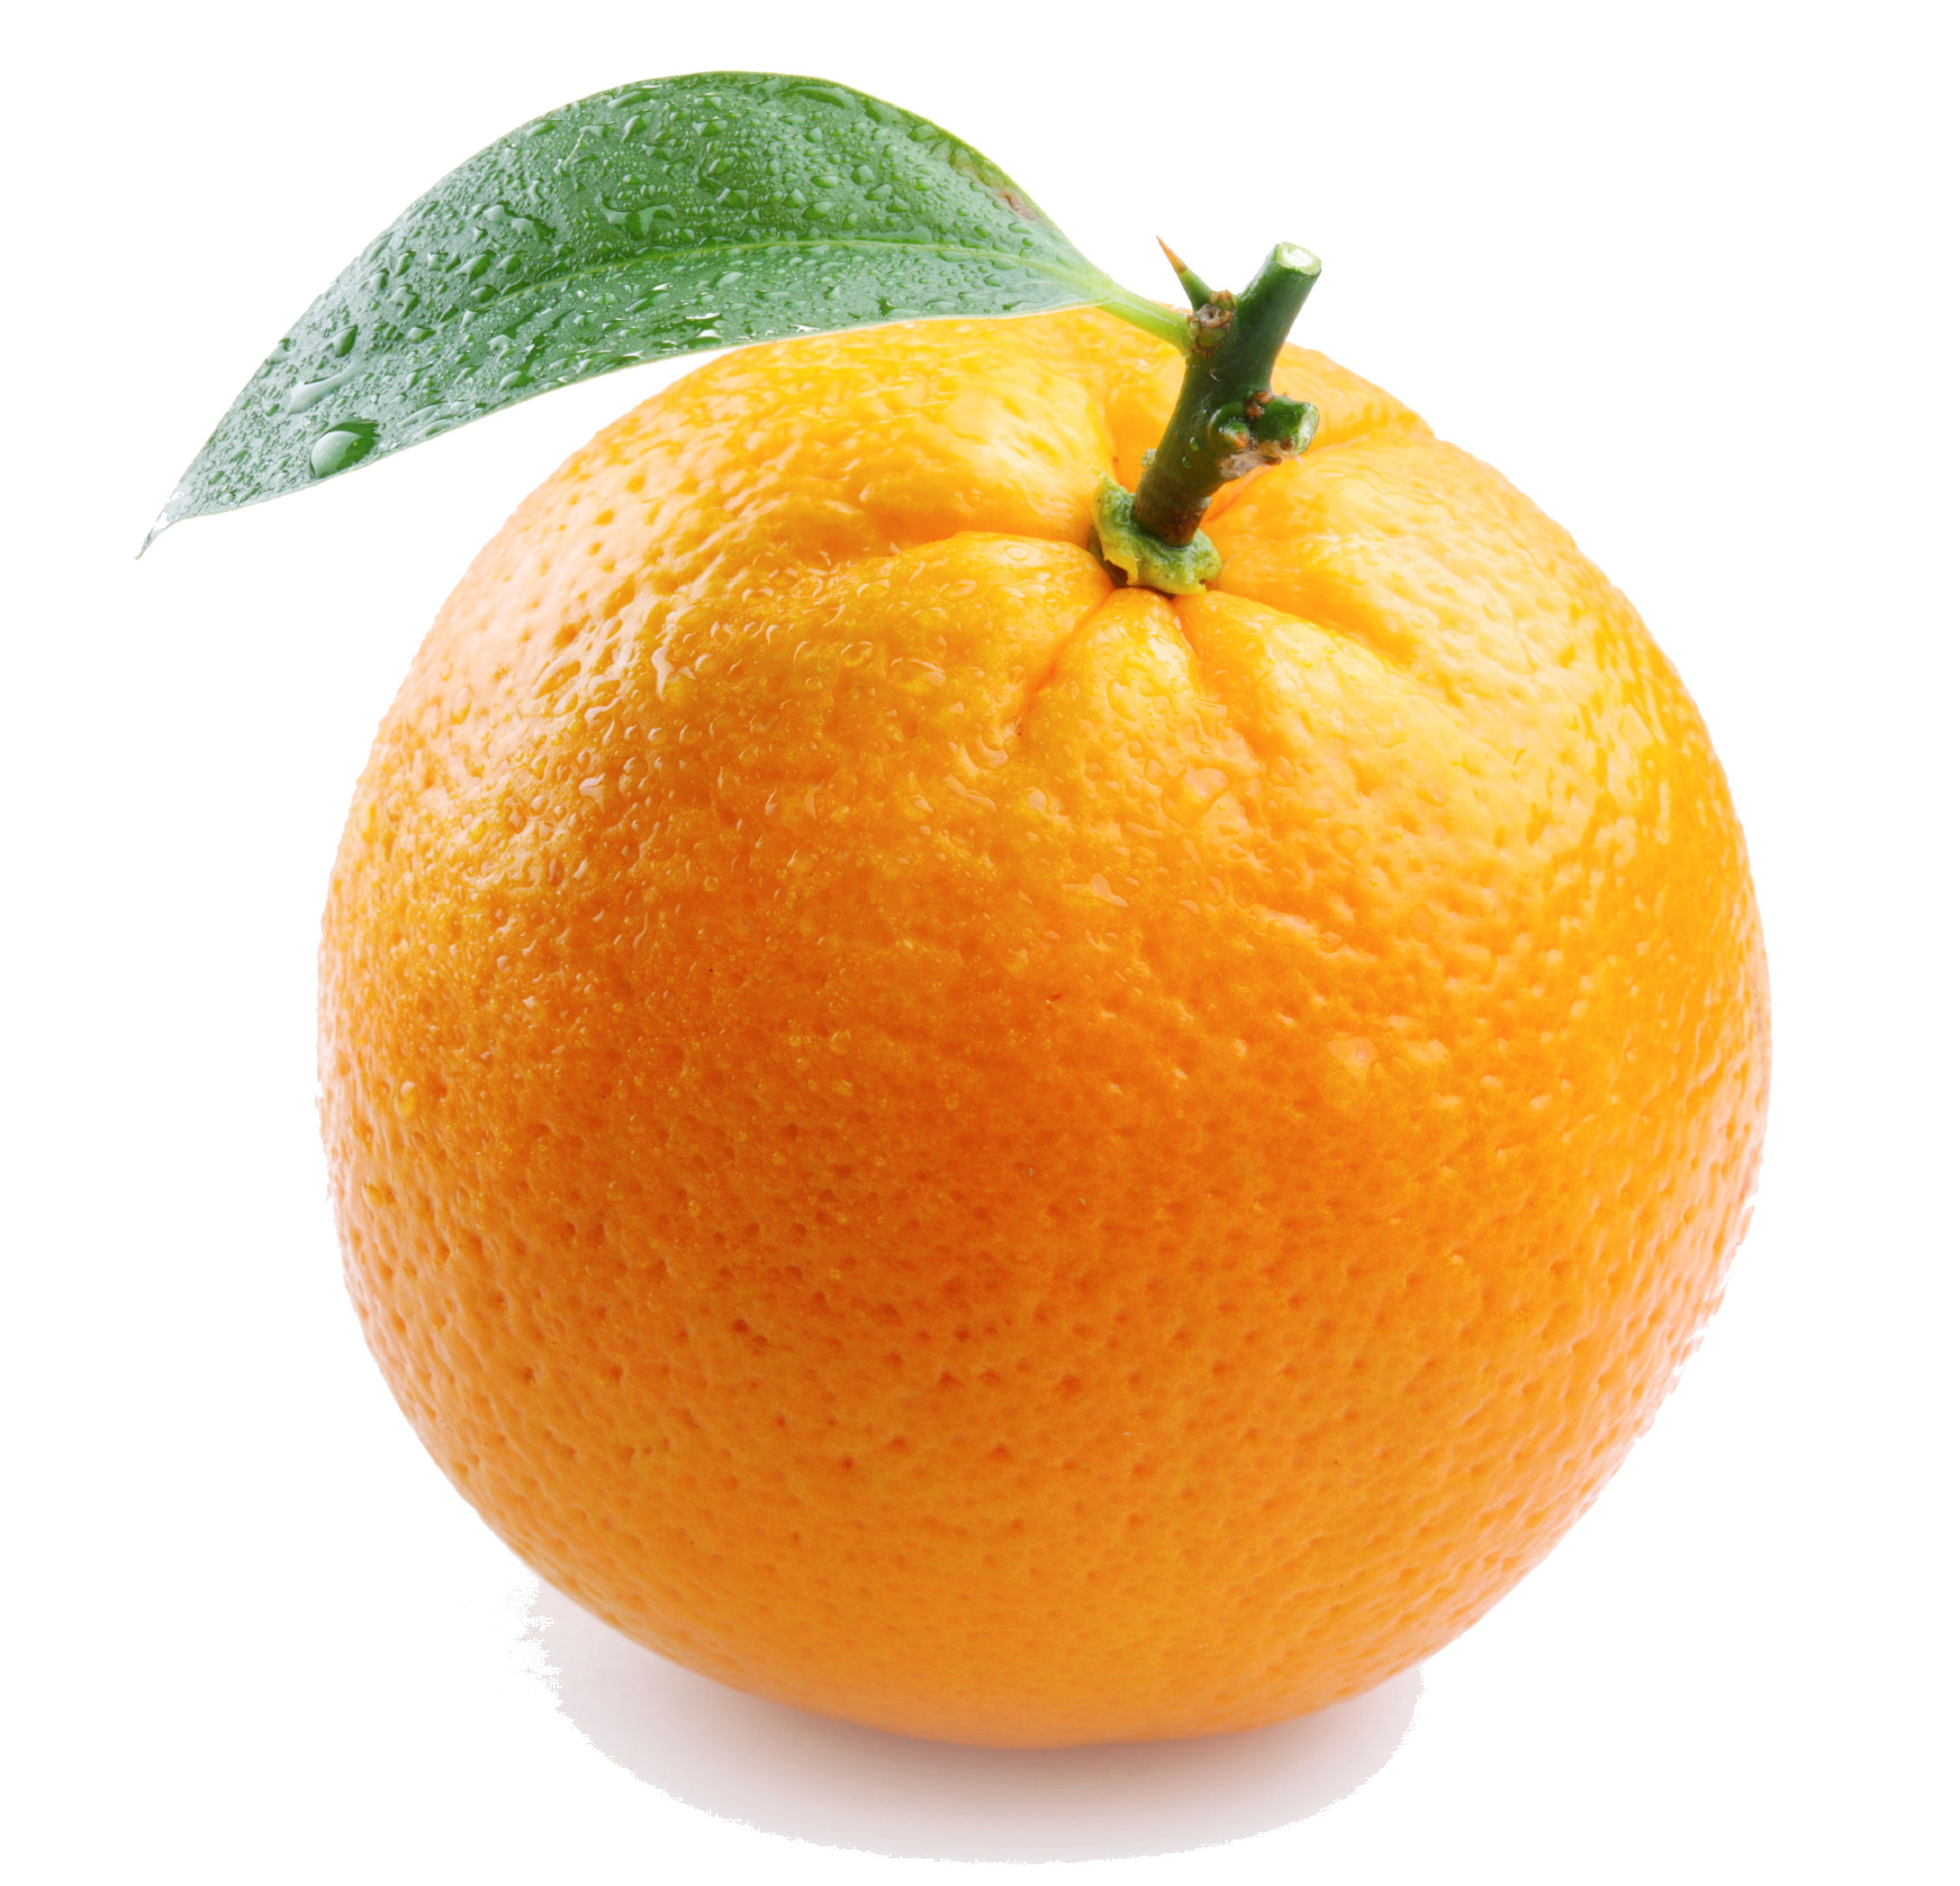
\includegraphics[width=\linewidth]{images/fruits/arancia.jpg}
  \caption{Arancia}
\end{subfigure}\hfill
\begin{subfigure}[t]{0.30\textwidth}
  \centering
  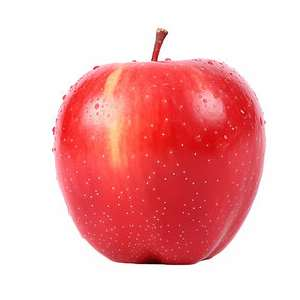
\includegraphics[width=\linewidth]{images/fruits/mela.jpg}
  \caption{Mela}
\end{subfigure}\hfill
\begin{subfigure}[t]{0.30\textwidth}
  \centering
  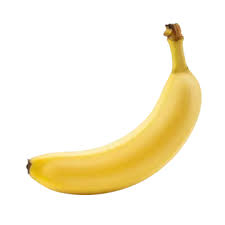
\includegraphics[width=\linewidth]{images/fruits/banana.jpg}
  \caption{Banana}
\end{subfigure}

\caption{Foto di frutta fresca in griglia 1x3.}
\label{fig:fruit_images1x3}
\end{figure}
\section{Griglia 2x2}
Ecco un esempio di una griglia di immagini, come mostrato in Figura \ref{fig:fruit_images2x2}.
\begin{figure}[H]
\centering

% --- First row ---
\begin{subfigure}[t]{0.45\textwidth}
  \centering
  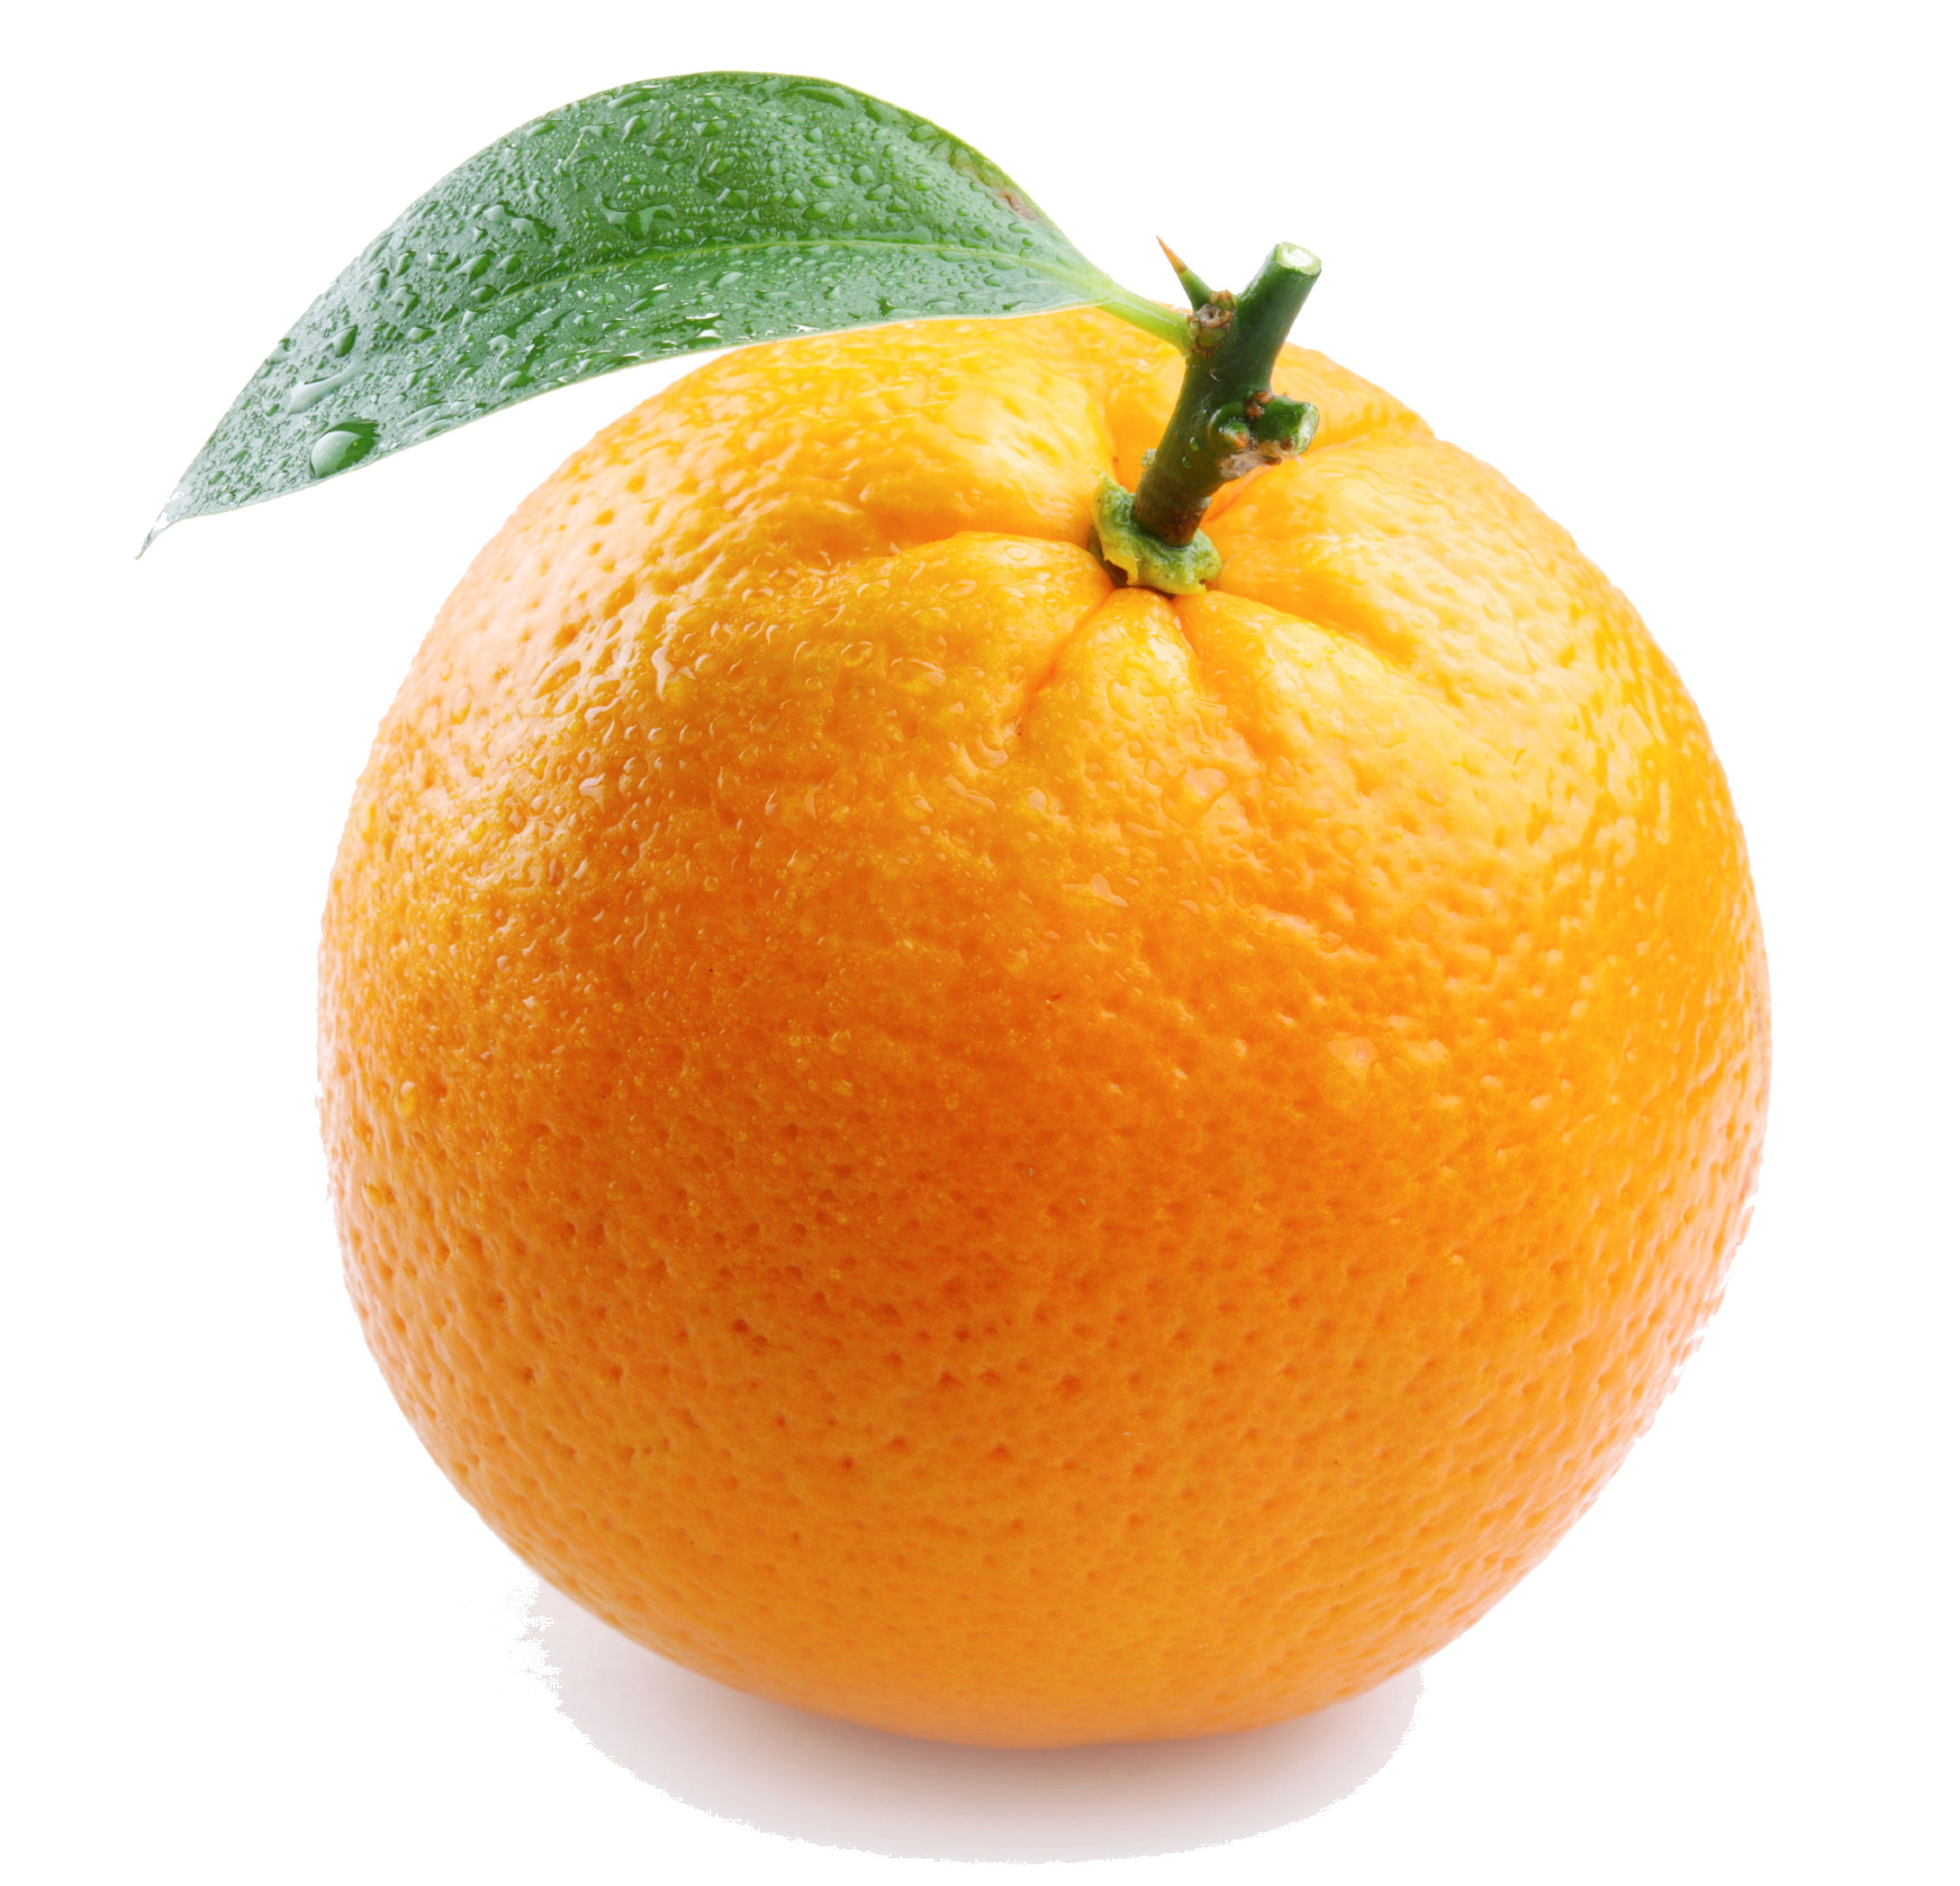
\includegraphics[width=\linewidth]{images/fruits/arancia.jpg}
  \caption{Arancia}
\end{subfigure}\hfill
\begin{subfigure}[t]{0.45\textwidth}
  \centering
  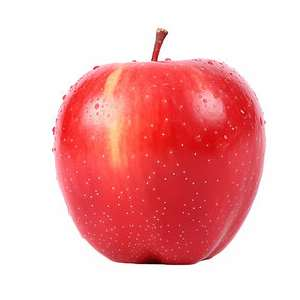
\includegraphics[width=\linewidth]{images/fruits/mela.jpg}
  \caption{Mela}
\end{subfigure}



% --- Second row ---
\begin{subfigure}[t]{0.45\textwidth}
  \centering
  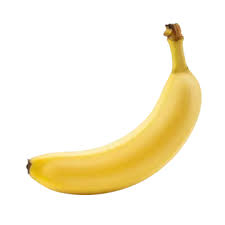
\includegraphics[width=\linewidth]{images/fruits/banana.jpg}
  \caption{Banana}
\end{subfigure}\hfill
\begin{subfigure}[t]{0.45\textwidth}
  \centering
  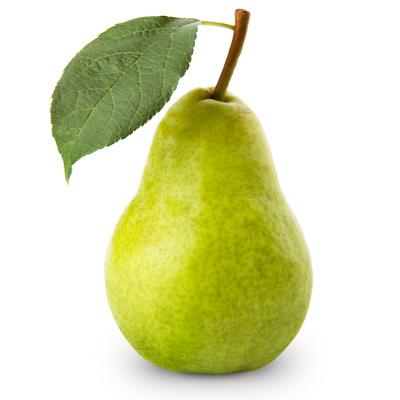
\includegraphics[width=\linewidth]{images/fruits/pera.jpg}
  \caption{Pera}
\end{subfigure}

\caption{Foto di frutta fresca in griglia 2×2.}
\label{fig:fruit_images2x2}
\end{figure}

\section{Esempio di Tabella Complessa}

\renewcommand{\arraystretch}{1.2}


\setlength{\tabcolsep}{3pt}

\begin{table}[tb]
\centering

\caption{Analisi comparativa di diversi frutti combinando vari metodi di maturazione, provenienze e punti di vista. Le Run ID rappresentano differenti esperimenti su raccolti.}
\label{tab:complex_table}


\begin{adjustbox}{width=0.9\textwidth}
\begin{tabular}{ccc*{11}r}
\toprule
\multirow{2}{*}[-5pt]{\rotatebox{90}{\textbf{Score}}} & 
\multirow{2}{*}[-3pt]{\rotatebox{90}{\textbf{Prov.}} } & 
\multirow{2}{*}[-12pt]{\rotatebox{90}{\textbf{Frutto}}} & 
\multicolumn{11}{c}{\textbf{Raccolti}}\\
\cmidrule(lr){4-14}
 &  &  & 
\makecell[c]{\rotatebox{90}{\textbf{R1}}} & 
\makecell[c]{\rotatebox{90}{\textbf{R2}}} & 
\makecell[c]{\rotatebox{90}{\textbf{R3}}} & 
\makecell[c]{\rotatebox{90}{\textbf{R4}}} & 
\makecell[c]{\rotatebox{90}{\textbf{R5}}} & 
\makecell[c]{\rotatebox{90}{\textbf{R6}}} & 
\makecell[c]{\rotatebox{90}{\textbf{R7}}} & 
\makecell[c]{\rotatebox{90}{\textbf{R8A}}} & 
\makecell[c]{\rotatebox{90}{\textbf{R8S}}} & 
\makecell[c]{\rotatebox{90}{\textbf{R9}}} & 
\makecell[c]{\rotatebox{90}{\textbf{R10}}} \\
\midrule

% ===============================================================
% PRIMA SEZIONE: Dolcezza 
% ===============================================================
\multirow{6}{*}{\rotatebox{90}{\textbf{Dolcezza}}}
& \multirow{2}{*}{\rotatebox{90}{Tutti}} & Mela & 87.23 & 88.01 & 87.44 & 86.99 & 88.12 & 87.55 & 88.23 & 87.66 & 88.42 & 88.09 & 87.77 \\
& & Banana & 91.31 & 92.05 & 91.74 & 91.92 & 90.84 & 92.18 & 91.95 & 92.02 & 91.85 & 91.99 & 91.88 \\
\cmidrule(lr){2-14}
& \multirow{2}{*}{\rotatebox{90}{Tropic.}} & Ananas & 84.45 & 85.02 & 84.60 & 84.99 & 84.25 & 85.15 & 84.79 & 84.92 & 85.11 & 84.85 & 84.88 \\
& & Mango & 90.12 & 90.89 & 91.10 & 90.67 & 90.33 & 91.21 & 90.97 & 91.03 & 91.30 & 90.95 & 91.12 \\
\cmidrule(lr){2-14}
& \multirow{2}{*}{\rotatebox{90}{Mediter.}} & Arancia & 88.44 & 89.11 & 88.99 & 89.23 & 88.51 & 89.34 & 89.28 & 89.21 & 89.43 & 89.15 & 89.32 \\
& & Limone & 72.62 & 73.40 & 73.88 & 72.95 & 72.50 & 73.91 & 73.65 & 73.75 & 73.84 & 73.70 & 73.78 \\
\midrule

% ===============================================================
% SECONDA SEZIONE: Succosità 
% ===============================================================
\multirow{9}{*}{\rotatebox{90}{\textbf{Succosità}}}
& \multirow{3}{*}{\rotatebox{90}{Tutti}} & Mela & 65.42 & 67.19 & 66.85 & 67.00 & 65.99 & 67.45 & 67.11 & 67.38 & 67.80 & 67.21 & 67.43 \\
& & Banana & 78.84 & 79.11 & 79.67 & 79.40 & 78.72 & 79.91 & 79.63 & 79.85 & 80.10 & 79.74 & 79.87 \\
& & Uva & 82.17 & 82.69 & 82.33 & 82.50 & 82.02 & 82.91 & 82.65 & 82.84 & 83.05 & 82.73 & 82.91 \\
\cmidrule(lr){2-14}
& \multirow{3}{*}{\rotatebox{90}{Tropic.}} & Mango & 85.15 & 85.44 & 85.98 & 85.67 & 85.01 & 86.11 & 85.79 & 85.92 & 86.22 & 85.83 & 85.96 \\
& & Papaya & 74.83 & 75.02 & 75.37 & 75.14 & 74.76 & 75.49 & 75.23 & 75.40 & 75.60 & 75.28 & 75.39 \\
& & Ananas & 77.04 & 77.49 & 77.71 & 77.31 & 77.05 & 77.80 & 77.58 & 77.66 & 77.93 & 77.60 & 77.74 \\
\cmidrule(lr){2-14}
& \multirow{3}{*}{\rotatebox{90}{Mediter.}} & Arancia & 81.90 & 82.30 & 82.65 & 82.49 & 81.87 & 82.76 & 82.52 & 82.68 & 82.95 & 82.59 & 82.70 \\
& & Limone & 61.35 & 61.88 & 62.09 & 61.95 & 61.24 & 62.22 & 62.05 & 62.17 & 62.44 & 62.10 & 62.26 \\
& & Pompelmo & 68.75 & 69.21 & 69.58 & 69.37 & 68.80 & 69.83 & 69.65 & 69.70 & 69.99 & 69.68 & 69.82 \\
\bottomrule


\end{tabular}
\end{adjustbox}
\vspace{-10pt} 
\end{table}




